\documentclass{article}
\usepackage{graphicx}
\usepackage{listings}
\usepackage{color}
\usepackage[margin=1.2in]{geometry}
\usepackage{courier}
\usepackage{float}
\usepackage[toc,page]{appendix}
\usepackage{amsmath}
\usepackage{hyperref}
\usepackage{setspace}
\doublespacing
\large

\definecolor{codegreen}{rgb}{0,0.6,0}
\definecolor{codeblack}{rgb}{0,0,0}
\definecolor{codered}{rgb}{0.867,0,0}
\definecolor{backcolour}{rgb}{ 0.95,0.95,0.95}
\definecolor{codeorange}{rgb}{1,0.447059,0}
\definecolor{codegrey}{rgb}{0.1, 0.1, 0.1}
\definecolor{codeblue}{rgb}{0.29, 0.52, 0.56}
\lstdefinestyle{mystyle}{
    basicstyle=\ttfamily\color{codeblack},
    backgroundcolor=\color{backcolour},   
    commentstyle=\color{codered},
    keywordstyle=\color{codeorange},
    numberstyle=\color{codeblack},
    stringstyle=\color{codegreen},
    breakatwhitespace=false,         
    breaklines=true,                 
    captionpos=b,                    
    keepspaces=true,                 
    numbers=left,                    
    numbersep=10pt,                  
    showspaces=false,                
    showstringspaces=false,
    showtabs=false,                  
    tabsize=3
}
 
\lstset{style=mystyle}

\begin{document}
\title{LIN3012 - Data-Driven Natural Language Processing}
\author{Daniel Cauchi}
\date{}
\maketitle

%\tableofcontents

\section{Introduction}
In this report, the task of Gender Identification on a Blog Corpus is implemented trough the use of Natural Language Processing techniques. The goal is to build a classifier which is able to recognize the differences in writing style between male and female writers. Usually, the issue of gender bias is one which researchers try to avoid, however in this case the opposite is required, where the features will be chosen to amplify this bias. The problem is to find the ideal features which will allow the generated model to discriminate best between male and female writers. For this approach, any feature which is related to topic is avoided, purely focusing on the style of writing. This is particularly difficult because the aim is to try and find similarities across an entire group of authors, because while individuals may have their own style of writing, it is more difficult to generalise the style of a set of people \cite{3}.


The solution to the gender identification problem has applications in areas such as forensics \cite{2, 6} and cyber criminal analysis \cite{1}, so the identity of a suspect may be narrowed down to one gender. Another application is in marketing \cite{6}, to find the demographic of some outlet.

The following chapters will discuss previous work done in this area, a description of the corpus in question, the approach taken to solve this problem and an evaluation on the model built.

\section{Previous Work}
The area of text categorization is highly studied and hence many works have been presented, however an optimal feature set hs not yet been published \cite{1}. This may be due to different domains having different features or due to the complexity of the problem. \cite{1} Uses RNN models for author identification. A particular emphasis is made on GloVe vectors. This method extracts both context, since it uses the actual words, as well as style, due to the RNN storing the sequence and hence the particular order in which the words are used. For this work however, context will not be taken into account, hence there is no use of topic specific words.

In \cite{3}, the authors of fictional and non-fictional works has been studied. It was noted that the main distinguishing features are different between the two domains. It was discovered that certain function words as well as parts-of-speech(POS) tags can be used to discriminate between the two genders in both domains. In this project, both of these feature sets are used applied to the blogging domain.

\cite{4} applies the task of gender identification for the e-mail domain. In this work, the language background of the author is also classified. It is stated that females tend to use more expressive language. These words include those such as "terribly" and "dreadful". In this project, these are accounted for by taking into account words ending with certain suffixes. A general distinction between the styles of men and females is that while males' conversation tend to prefer 'report-talk' while females prefer 'rapport-talk'.

\cite{2} use the same corpus as this project and define the state of the art of this task. They claim that women write in a style which is more involved, meanwhile men prefer writing which give more information, which is similar to the 'report' and 'rapport' talk discussed by \cite{4}. Important features such as the number of URL links and use of pronouns are discussed, and some of these will be used within this project \cite{2} also uses the topics and individual words of the posts. This is something which this work will avoid, to try and see how well the gender can be predicted using purely style based features without the bias of topic. The observation that style changes as the age changes is also made. This means that as age differs, the style between the gender also varies and blend into each other, making it more difficult to extract gender based purely off of stylistic features.
\section{Data and Methodology}

\subsection{The Corpus}
The corpus used is the Blog Authorship Corpus by \cite{2}. This is a corpus containing posts from 19320 blogs, with 9660 of them being male and another 9660 of them being female. In total there are 344773 male posts and 335010 posts. Other meta-data includes the age range of the bloggers and their star sign. These will not be considered. Other observations on the data include that there are some null posts, which will be pruned later on. Furthermore, some blogs are pure spam, with posts containing garbage such as advertisements or non-sense sentences. These will act as noise in the data. The individual posts were trimmed from trailing spaced and new lines were replaced by fullstops.


\subsection{Feature Extraction and Filtering}
The following 'general' features were extracted from the corpus for each post: Word Count, Sentence Count, Average Word Length, Average Sentence Length, Number of Unique Words/Word Count, Number of URLs/Word Count. The number of words ending with the following suffixes were also counted and divided by the Word Count: able, al, ful, ible, ic, ive, less, ly, ous. This list was obtained from \cite{4} The reason they were divided by the Word Count is because the length of a post may affect the frequency of words in general, hence the features are normalized by this value. It is important to note that the words considered in this case do not include any punctuation.

A few vocabularies were created to extract some important words and bi-grams with regards to the posts. Prior to this however, the posts were split into a train and test set. This was done by first sorting the dataset by file name in ascending order, and getting the number of posts by each author. Then the train set was made to contain round 80\% of each gender. This was made so that author who is in the train set can be in the test set. Precisely, the training set contains the first 7728 male blogs (270106 posts) and the first 7148 female blogs (269911 posts), so that the number of posts balance out. The rest was left for testing.

The posts were then converted twice, once as POS tags using the NLTK averaged perceptron tagger and once as bleached text \cite{5}. In this project's case, the bleaching technique used was to replace consonants with the letter C and vowels with the letter V. Bleaching allows for abstracting the word itself to avoid content (and language) bias, but rather focusing on the form of the word. The hypothesis here is that men and women use different word forms when writing. After the conversion process, a vocabulary of bi-grams and their sum of normalized counts is generated on the train set. Bi-grams were chosen over uni-grams to account for ordering and they were chosen over tri-grams because posts tend to be short, hence these might have ended up being too sparse. The sum of normalized counts, which will be abbreviated to SNC from now on, is the sum of the counts of an item within a document, divided by the total items of that type in that document, for all documents. This is used so that the length of the posts does not skew the counts, such that lengthier posts would have bigger weight. So for an item x, the SNC of x over all the documents(the posts, in this case) D is: 

\[SNC(x) = \sum_{d \in D} \frac{number\, of\, times\, x\, occurs\, in\, d}{number\, of\, items\, with\, the\, same\, type\, of\, x\, in\, d}\]

2 values for SNC were generated on the train set for each POS bi-gram and bleached bi-gram. The first value is the SNC over the male written documents and the second on the second on the documents written by females. This resulted in 1,692 POS bi-grams and 2,010,167 bleached bi-grams. These were then filtered by removing those with total SNC (SNC over the male written documents + SNC over the female written documents) of 100 so that the chances of them appearing in the test set as well is high, therefore avoiding sparseness in the data. These were then sorted by their entropy and the top 50  with the least entropy (highest information gain) from each group was taken, so that in the end 50 POS bi-grams and 50 bleached bi-grams were obtained as features. This was done to not have too many unnecessary features.

The final selected POS bigrams were the following: 'VB VBP', '. .', 'NNP NNPS', 'JJ VBP', 'NNP ``', 'NNP TO', 'DT NNP', 'NNP MD', 'NNP )', '. )', 'CD NNP', '. NN', 'NNP NNS', ') PRP', 'NN VBP', 'PRP CC', '( NNP', '`` DT', 'NNP (', 'PRP WRB', 'NNP VBZ', 'POS NNP', '( CD', '`` NNP', 'IN NNP', 'NNS VBZ', 'NNP CD', '. VBN', 'JJ PRP', 'VBG NNP', 'CD )', 'CD ,', 'VBP VBP', 'NNP DT', 'VBN VBN', '. (', 'NNP IN', 'NNP :', 'CD :', ': NNP', 'VBP PRP', 'VBP WP', 'PRP PRP', 'PRP NN', 'VBP WRB', 'PRP .', 'WP NN', 'DT ``', 'PRP VB', 'VBN DT'.

The final selected bleached bi-grams were the following: 'CVV ?', 'VCCCVCC CVCCVC', '-- --', 'VCCCVCC CVCCVCC', '! V', 'VCCCVCC CCCC', 'VCV CVV', 'CVV !', 'CCCC :', '! CV', '! !', '! CVC', '. :', 'CVCCC !', '! )', '! VCC', '? ?', '! VC', 'CV !', '! CVCV', 'CVCV VCCCVCC', 'CC VCCCVCC', 'CVC !', 'CCV VCCCVCC', 'VC VCCCVCC', '? !', 'VC !', 'CVCC !', 'CCVC VCCCVCC', 'VCCCVCC CVCVC', '! VCCCVCC', 'CC CVVCC', 'CCV ``', "CCV '" ',CVCVC !' ',! CCVC' ',CVCV !' ',CVCVVC VC' ',! CVCC' ',VCCCVCC CVCC' ',CVCVVCV V' ',: V' ',: )' ',: ``' ',CVVC !' ',V VC' ',CCV CVCCVCV' ',VCCCVCC CVVC' "CV '," 'CCV CVCVCVC'.

The final set of features were function words. The entire set of considered function words consisted of 277 function words obtained from \url{https://semanticsimilarity.files.wordpress.com/2013/08/jim-oshea-fwlist-277.pdf}. These were pruned much the same way as the bi-grams. Those with a total SNC of 50 or more were taken, then the top 50 of those with least entropy were chosen. It is important to note that when using SNCs, the words used were generated by 'word\textunderscore tokenize' from nltk, so punctuation was considered.

The final selected function words were the following: i, even, under, mine, most, of, shall, do, second, these, by, some, because, did, its, an, often, during, when, as, few, inside, near, too, also, together, between, rather, never, someone, may, their, everything, always, yes, he, which, has, my, so, etc, am, me, sometimes, myself, her, alone, she.

After the features were decided, feature extraction was done for each document. When it came to the bi-grams and function word counts, these were divided by the total number of bigrams or words in that document as well. 

\subsection{Model Creation}
2 models were created using scikit-learn \cite{scikit-learn}. The first is a Logistic Regression model and was used as a baseline. The second is a multi-layer-perceptron with 1 hidden layer of 265 nodes (the total number of features + 100). Prior to training, the hyperparameters of the models were tuned using scikit-learn's random search, which is similar to grid search but does not search trough all combinations. This evaluates the models created using a cross validation technique. Note: this search was made on 10,000 of the train set. After the best hyperparameters are found, the classifier is fit on the entire train set and tested on the test set.
\section{Results and Evaluation}
The confusion matrix of the baseline model can be seen in figure \ref{fig:baseline} while that of the main model can be seen in figure \ref{fig:main}. The accuracy of the baseline ended up being 60\% while that of the main model ended up being _\%. These results are very similar and the base on the fact that the overall accuracy is above 50\% shows that some form of pattern was found. However, this is terrible, compared to the state of the art presented in \cite{2} which achieved an overall accuracy of 80.1\%. Next, the reasons as to why these results may have occurred are discussed.

\begin{figure} \label{fig:baseline}
	\centering
	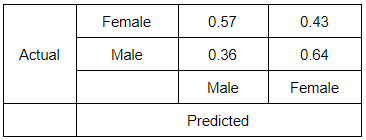
\includegraphics[width=0.7\textwidth]{Images/LR-CM.png}
	\caption{Logistic Regression Model Confusion Matrix}
\end{figure}

\section{Conclusion}

\pagebreak

\bibliography{main}
\bibliographystyle{ieeetr}

\pagebreak

\chapter*{Appendix}\addcontentsline{toc}{section}{Appendix}

\section*{Plagiarism Form}
\begin{figure}[H]
	\centering
	\includegraphics[width=0.7\textwidth]{Images/plagiarismform.png}
\end{figure}

\pagebreak

\section*{Completion Form}
\begin{table}[h]
	\begin{tabular}{|l|l|}
		\hline
		\textbf{Item}                                     & \textbf{Completed} (Yes/No/Partial) \\ \hline
		&                            \\ \hline
		SVM technical discussion     & Yes                        \\ \hline
		A good comparison to alternative methods                  & Yes                        \\ \hline
		Artifact                  & Yes                        \\ \hline
		Experimentation with different SVM parameters                  & Yes                        \\ \hline
		Experiments and their evaluation & Yes                        \\ \hline
		Overall conclusions           & Yes                        \\ \hline
	\end{tabular}
\end{table}

\end{document}